% =============================================================================
% Politely: rewriting impolite sentences with a seq2seq model
% NLP course project - 2-page report
% Compile with pdflatex (Overleaf or TeX Live). Figures are in figures/.
% =============================================================================
\documentclass[10pt,a4paper]{article}

\usepackage[utf8]{inputenc}
% (default Computer Modern fonts)
\usepackage[a4paper,margin=1.45cm,top=1.3cm,bottom=1.5cm]{geometry}
\usepackage{amsmath,amssymb}
\usepackage{graphicx}
\usepackage{booktabs}
\usepackage{tabularx}
\usepackage{xcolor}
\usepackage{titlesec}
\usepackage{caption}
\usepackage{pifont}
\usepackage{microtype}
\usepackage[hidelinks]{hyperref}

\definecolor{teal}{HTML}{176F63}
\titleformat{\section}{\normalsize\bfseries\color{teal}}{\thesection.}{0.4em}{}
\titlespacing*{\section}{0pt}{5pt}{2pt}
\captionsetup{font=footnotesize,labelfont=bf,skip=2pt}
\setlength{\parindent}{0pt}
\setlength{\parskip}{2.5pt}
\setlength{\textfloatsep}{6pt}
\setlength{\intextsep}{4pt}
\pagestyle{plain}

\newcommand{\cmark}{\textcolor{teal}{\ding{51}}}
\newcommand{\xmark}{\textcolor{red!70!black}{\ding{55}}}
\newcommand{\tok}[1]{\texttt{\small #1}}

\begin{document}

\begin{center}
  {\Large\bfseries Politely: rewriting impolite sentences with a seq2seq model}\\[3pt]
  {\small \textbf{Ikram Saidane} $\cdot$ NLP course project $\cdot$ November 2026\\
  Code, notebook, trained models and interface: \url{https://github.com/Ikram-Saidane/politely-seq2seq}}
\end{center}
\vspace{-6pt}

% -----------------------------------------------------------------------------
\section{Introduction}
For this project I chose to turn impolite English sentences into polite ones, for example
\emph{``Send me the report now.''} $\rightarrow$ \emph{``Could you please send me the report as soon as possible?''}.
I liked this task because the output has to change the tone but \textbf{keep the meaning}: the person,
the object and the time must stay the same. It is a sequence-to-sequence problem, so I built an
encoder--decoder in PyTorch from scratch (no pretrained model). A good output must be \textbf{polite},
\textbf{faithful} to the input and \textbf{fluent}.

% -----------------------------------------------------------------------------
\section{Related concepts}
The \textbf{encoder} (an LSTM) reads the sentence word by word and the \textbf{decoder} (another LSTM)
writes the new sentence one word at a time, using the previous word. With only the last encoder state,
the decoder forgets long inputs, so I added \textbf{Bahdanau attention}: at each step the decoder looks
at all input words and takes a weighted average of them. Finally I added a \textbf{copy mechanism}
(pointer-generator): the model can either generate a word from the vocabulary or copy a word of the
input, which is useful for names and numbers.

% -----------------------------------------------------------------------------
\section{Dataset}
I did not want to use public corpora like ParaDetox because they contain many insults. So I wrote a
small Python program (\texttt{generate\_dataset.py}) that combines situations, people, objects and
phrasings that I wrote by hand, in \textbf{9 balanced categories} (request, reminder, refusal,
criticism, complaint, disagreement, question, stop, announcement), with no offensive words. It is
reproducible (seed 42). Every input has 2 polite references in train, 3 in valid/test/test\_unseen and
1 in the hand-written set, and the splits are made \textbf{by content}, so no sentence appears twice.

My \textbf{first version} (\texttt{data\_v1/}) was a mistake in some ways: it only talked about office
life (1,371 words) and had incoherent pairs such as \emph{``Move your car out of the library''} or
\emph{``Call Sarah back. Call it today.''}. The models trained on it reached only 0--1\,\% success on
sentences I wrote myself. I \textbf{improved} it: I removed the incoherent pairs and widened the
vocabulary to everyday life (1,805 words). The comparison is in \texttt{reports/dataset\_v1\_vs\_v2.json}.

\begin{center}
\small
\begin{tabularx}{\linewidth}{@{}lXXXXX@{}}
\toprule
Split & train & valid & test & test\_unseen & challenge \\
\midrule
Inputs / pairs & 14,400 / 28,800 & 1,350 / 4,050 & 1,350 / 4,050 & 900 / 2,700 & 72 / 72 \\
Used for & training & choosing models & same phrasings & \textbf{new phrasings} & \textbf{my own sentences} \\
\bottomrule
\end{tabularx}
\end{center}

% -----------------------------------------------------------------------------
\section{Preprocessing}
I normalise Unicode, lowercase the text (the case is put back for display), separate punctuation
(the \emph{?} matters a lot here) and split into words, keeping contractions like \emph{don't}. The
vocabulary is built \textbf{only on train} with words seen at least twice, plus
\tok{<PAD> <SOS> <EOS> <UNK>}. Sentences are padded in a batch and cut at 40 tokens.
Example: \emph{close the window now .} $\rightarrow$ \tok{390 4 573 58 5 2}.

% -----------------------------------------------------------------------------
\section{Architecture}
Embeddings of size 128 $\rightarrow$ \textbf{LSTM encoder} (hidden 256) $\rightarrow$
\textbf{attention} ($e_j = v^\top \tanh(W_1 h_j + W_2 s)$, softmax, context vector) $\rightarrow$
\textbf{LSTM decoder} fed with the previous word and the context $\rightarrow$ linear layer + softmax
over the 1,805 words, until \tok{<EOS>}. For copying, $p_{gen} = \sigma(w \cdot [c; s; e])$ decides
between generating and copying. I compared: \textbf{A} without attention (1.30\,M parameters),
\textbf{B} with attention (1.66\,M), \textbf{C} with copy (1.67\,M), and variants D (GRU), E (hidden
128 or 512) and F (teacher forcing 0.5).

% -----------------------------------------------------------------------------
\section{Training}
Cross-entropy on tokens (padding ignored), Adam with lr $10^{-3}$ (halved when validation stops
improving), batch 64, dropout 0.3, gradient clipping at 1.0, early stopping with patience 3 and at
most 30 epochs. Everything ran on CPU, about 1 to 2 minutes per epoch. Before each real training I
checked that the model could \textbf{memorise 40 pairs} (model C: loss 5.7 $\rightarrow$ 0.11), which
helped me find bugs early.

% -----------------------------------------------------------------------------
\section{Experimental results}
I count an output as a \textbf{success} if a small politeness classifier (logistic regression) finds
it polite, \textbf{all content words are kept} and there is no repetition. I also report BLEU. I chose
the model and the decoding (greedy, beam 3/5, sampling, top-k) on the validation set: the final system
is \textbf{C with beam search 5}.

\noindent\begin{minipage}{\linewidth}
\centering\small
\begin{tabularx}{\linewidth}{@{}Xcccc@{}}
\toprule
System & test & test\_unseen & challenge & BLEU (test) \\
\midrule
Copy baseline / rule-based baseline & 0.000 / 0.125 & 0.034 / 0.253 & 0.000 / 0.097 & 47.5 / 48.2 \\
A $\cdot$ LSTM, no attention & 0.845 & 0.350 & 0.111 & 74.2 \\
B $\cdot$ + attention & 0.912 & 0.582 & 0.222 & 77.2 \\
\textbf{C $\cdot$ + copy, beam 5 (final)} & \textbf{0.999} & \textbf{0.787} & \textbf{0.764} & 77.2 \\
C, \emph{acceptable} in human evaluation$^{*}$ & 0.975 (40) & 0.375 (40) & 0.528 (72) & -- \\
\bottomrule
\end{tabularx}\\[2pt]
{\footnotesize $^{*}$ One annotator only; the labels were produced with the help of an AI assistant.}
\end{minipage}\vspace{4pt}

Attention makes training faster (best epoch 24 $\rightarrow$ 5) and keeps more content, but the
\textbf{biggest gain comes from copying} (challenge 0.22 $\rightarrow$ 0.76). A bigger or smaller
model, a GRU or teacher forcing 0.5 did not help (0.91--0.93 on test), and word dropout even made
results worse. Without copy, the models overfit slightly (A: training loss 0.11 vs validation 0.17),
but early stopping keeps the best epoch; with copy (C), both losses stay equal ($\approx$ 0.10).

\begin{figure}[h]
  \centering
  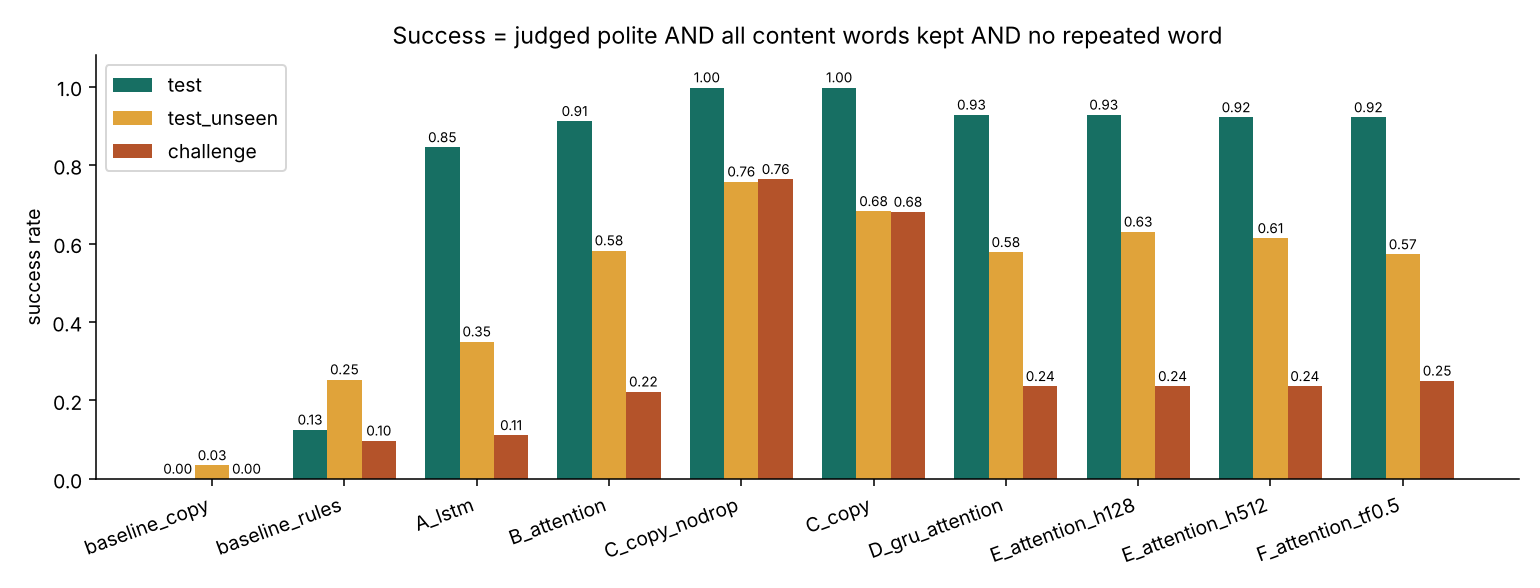
\includegraphics[width=0.74\linewidth]{figures/results_success.png}
  \caption{Success rate of each system on the three test sets.}
  \vspace{2pt}
  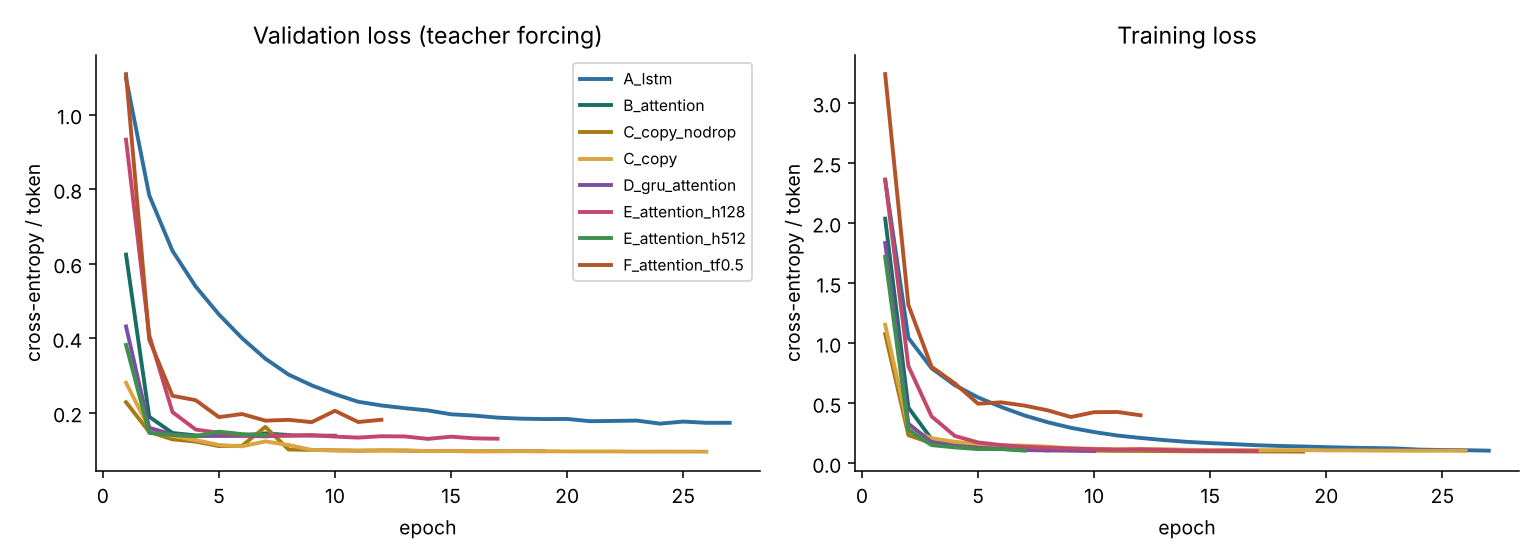
\includegraphics[width=0.70\linewidth]{figures/learning_curves.png}
  \caption{Validation and training loss of every model per epoch.}
\end{figure}

% -----------------------------------------------------------------------------
\section{Generated examples}
\begin{tabular}{@{}l@{\ }p{0.94\linewidth}@{}}
\cmark & \emph{Turn the music down.} $\rightarrow$ \emph{Could I ask you to turn the music down? Thank you!} \\
\cmark & \emph{You're wrong. Water boils at 100 degrees.} $\rightarrow$ \emph{Actually, I think water boils at 100 degrees. Could you double-check?} \\
\xmark & \emph{I won't lend you any more money.} $\rightarrow$ \emph{Would it be possible for you to lend you any more money?} (the meaning is reversed) \\
\xmark & \emph{You were supposed to pay the rent yesterday.} $\rightarrow$ \emph{\dots\ could you pay the rent yesterday?} (wrong tense). Both errors are counted as successes by the automatic metric, hence the human evaluation. \\
\end{tabular}

% -----------------------------------------------------------------------------
\section{Discussion}
The model learned the polite sentence \emph{frames} very well and copies the content reliably, but it
chooses the frame from a few cue words. When it meets a rude opening it has never seen, it copies it as
if it were content, and it does not adapt the grammar. The automatic score agrees with the human
evaluation on the test set but is too optimistic on my own sentences (0.76 vs 0.53).
\textbf{Limits:} a finite set of phrasings, a simple bag-of-words politeness classifier, a word-level
vocabulary. \textbf{Next steps:} more varied data, subword units (BPE), a Transformer with copy, and a
human evaluation with several annotators.

% -----------------------------------------------------------------------------
\section{Conclusion}
A small encoder--decoder trained from scratch can rewrite impolite sentences politely. Attention and
especially the copy mechanism keep the content (17\,\% $\rightarrow$ 53\,\% acceptable on my own
sentences), while a bigger model did not help and better data did. The main lesson for me: test the
model far from the training data and always check the metrics by hand.

\end{document}
